\documentclass[a4paper]{memoir}

\usepackage{style}      % Custom style

\bibliography{bibliography} %% in order for sublime to find bib refs 

\usepackage{kantlipsum} % Dummy text

\title{Components of the Hilbert scheme in $\P^{11}$}
\author
{
    Fredrik Meyer
}

 \includeonly
 {
    sections/abstract,
    sections/acknowledgements,
    sections/introduction,
    sections/preliminaries,
    sections/cp2_triangulation,
    sections/two_smoothings,
    sections/constructions
 }

\begin{document}

    \frontmatter        % Folios in Roman numerals, unnumbered chapters.

    \begin{titlingpage}
        \maketitle
    \end{titlingpage}

    \abstractintoc % Add abstract to Table of Contents  
%\abstractnum  % Format abstract like a chapter

\begin{abstract}
    %\noindent
    
After a preliminary chapter introducing concepts and definitions, we explore a connection between triangulations of $\C \P^2$ and degenerations of hyper-Kähler manifolds. Then we study the topology of the two smoothings of the affine cone over $\dP6$, and prove that they are topologically different by computing their singular cohomology groups. In the last chapter we construct new examples of smooth Calabi--Yau manifolds, and their respective mirrors.
\end{abstract}
    \chapter{Acknowledgements}


I am grateful to my advisor, Jan Christophersen, for the suggestion of this project, his unending enthusiasm, and his always open door. \newline

\noindent I thank my family (mamma, pappa, Therese, Lovise and Marie) for being there, for the love and support I got from them, and for reminding me that life is more than numbers. \newline

\noindent I want to thank Karoline Moe for her support when my motivation was low and her encouragement when my motivation was high. \newline

\noindent I am indebted to Martin Helsø for his instant \LaTeX\, support service and his typographical advice.\newline

\noindent Finally, I'd like to thank all the frequenters of the lunch area in the 6th floor of the Mathematics building. You are great people, and you all made it easier for me to work on my PhD.

    \tableofcontents    % Or \tableofcontents*
    \listoffigures
    \listoftables

    \chapter{Introduction}
\label{sec:intro}

\kant[4] % Dummy text

\section{Figures and Tables}

% Standalone with \input:
\begin{figure}[htbp]
    \centering
    \input{figures/ball}
    \caption[One ball]{One ball.}
\end{figure}

% Standalone with \includegraphics:
\begin{figure}[thbp]
    \centering
    \includegraphics{balls}
    \caption[Two balls]{Two balls.}
\end{figure}

% Todonotes:
\begin{figure}[hbp]
    \centering
    \missingfigure{Three balls.}
    \caption[Three balls]{Three balls.}
\end{figure}

\kant[5-6] % Dummy text

% Booktabs:
\begin{table}[htbp]
    \centering
    \begin{tabular}{cc}
        \toprule
        \textbf{Correct}               & \textbf{Incorrect} \\
        \midrule
        \( \varphi \colon X \to Y \)   & \( \varphi : X \to Y \)  \\[0.5ex]
        \( \varphi(x) \coloneqq x^2 \) & \( \varphi(x) := x^2 \)  \\
        \bottomrule
    \end{tabular}
    \caption[Colons]{Proper colon usage.}
\end{table}

% Tablefootnote and multirow:
\begin{table}[htbp]
    \centering
    \begin{tabular}{cc}
        \toprule
        \textbf{Correct}
        & 
        \textbf{Incorrect}
        \\
        \midrule
        \( -1 \) 
        & 
        -1
        \\[0.3ex]
        1--10
        &
        1-10
        \\[0.3ex]
        Birch--Swinnerton-Dyer\tablefootnote{It is now easy to tell that Birch and Swinnerton-Dyer are two people.} conjecture
        &
        Birch-Swinnerton-Dyer conjecture
        \\[0.3ex]
        The ball \dash which is blue \dash is round.
        &
        \multirow{ 2}{*}{The ball - which is blue - is round.}
        \\[0.3ex]
        The ball---which is blue---is round. 
        &
        \\
        \bottomrule
    \end{tabular}
    \caption[Dashes]{Proper dash usage.}
\end{table}

    \mainmatter         % Folios in Arabic numerals, numbered chapters.


    % \part{The First Part}
    \chapter{Preliminaries}
\label{sec:prelims}

\begin{enumerate}
	\item Stanley-Reisner schemes
	\item Toric geometry notation
\end{enumerate}

\section{Deformation theory}

Given a scheme $X_0$ over $\C$, a \emph{family of deformations} of $X_0$ is a flat morphism $\pi:\mathscr X \to (S,0)$ with $S$ connected such that $\pi^{-1}(0)=X_0$. If $S$ is the spectrum of an artinian $\C$-algebra, then $\pi$ is an \emph{infinitesimal deformation}. If $S=\Spec \C[\epsilon]/\epsilon^2$, then  $\pi$ is a \emph{first order deformation}. A \emph{smoothing of $X_0$} is a deformation such that the general fiber is smooth.

\section{Stanley-Reisner schemes}

\subsection{Simplicial complexes and Stanley--Reisner schemes}

Denote by $[n]$ the set $\{0,1,\ldots,n\}$, and by $\Delta_n$, the set of all subsets of $[n]$. This is the \emph{$n$-dimensional simplex}. A \emph{simplicial complex} $\K$ is a subset of $\Delta_n$ that is closed under the operation of taking subsets. The subsets of $\K$ are called \emph{faces}. A good reference is Stanley's green book \cite{stanley_green}.

Let $k$ be a field, and let $P_\K$ be the polynomial ring over $k$ with variables indexed by the vertices of $\K$. Then the \emph{face ring} or \emph{Stanley--Reisner ring} of $\K$ is the quotient ring $A_\K = P_\K/I_\K$, where $I_\K$ is the ideal generated by monomials corresponding to non-faces of $\K$. 

\begin{example}
Let $\K$ be the triangle with vertices $\{ v_1,v_2,v_3\}$. Its maximal faces are $v_1v_2, v_2v_3$ and $v_1v_3$. The Stanley--Reisner ring is $k[v_1,v_2,v_3]/(v_1v_2v_3)$.
\end{example}

The ideal $I_\K$ is graded since it is defined by monomials. This leads us to define the \emph{Stanley--Reisner scheme} $\P(\K)$ as $\Proj A_\K$. 

There is a correspondence between certain degenerations of toric varieties and so-called unimodular triangulations. \todo{define these}

Let $M$ be a lattice (by which we mean a free abelian group of finite rank). Let $\nabla \subset M_\Q = M \otimes_\Z \Q$ be a lattice polytope, and let $S_\nabla$ be the semigroup in $M \times \Z$ generated by the elements $(u,1) \in \nabla \cap M$. Then we define $\P(\nabla)=\Proj \C[S_\nabla]$, and call it the \emph{toric variety associated to $\nabla$}. 

By Theorem 8.3 and Corollary 8.9 in \cite{sturmfels}, there is a one-one correspondence between unimodular regular triangulations of $\nabla$ and the square-free initial ideals of the toric ideal of $\P(\nabla)$. 

\section{Toric geometry}
\label{sec:toricgeometry}

\todo{fill in as needed}

\section{Smoothings of Stanley--Reisner schemes}

Because many properties of varieties are easier read off their degenerations, it is an interesting problem to study smoothings of Stanley--Reisner-schemes, which are highly singular.

\begin{lemma}
\label{lemma:srcohom}
If $\K$ is a simplicial complex, then $H^i(\K;k) \simeq H^i(\P(\K),\OO_{\P(\K)})$.
\end{lemma}
\todo{Find a good proof for this. A reference could be \cite{eisenbud_graphcurves}}

\begin{lemma}
If $\K$ is a 3-dimensional simplicial sphere, then a smoothing of $X_0=\P(\K)$ will be Calabi--Yau.
\end{lemma}
\begin{proof}
Since $\K$ is a sphere, it follows from \ref{lemma:srcohom} that $H^i(X_0,\OO_X)=k$ for $i=0,3$, and zero for $i \neq 0,3$. It also \todo{How does triviality of the canonical sheaf follow?}
\end{proof}
    \chapter{Relation to triangulations of \texorpdfstring{$\C\P^2$}{CP2}}
\label{sec:cp2triangs}

This chapter will not contain any new results of any signifance, but is rather a report on an idea which led to the deliberations in the later chapters.

We explain a connection between the topological space $\C \P^2$ and hyper-Kähler manifolds.

\section{Introductory remarks} % (fold)

\subsection{Hyper-Kähler manifolds}
\label{sec:hyper_kähler_manifolds}

Among the known families of manifolds, hyper-Kähler manifolds are among the most elusive. One often divides manifolds into three types: those with positive, negative or trivial canonical class. Of those with trivial canonical class, two prominent types stand out: Calab--Yau-manifolds and hyper-Kähler manifolds.

\begin{definition}
A \emph{hyper-Kähler manifold} $X$ is a simply connected compact Kähler manifold such that $H^0(X, \Omega_X^2)$ is generated by a non-degenerate $\sigma: TX \times TX \to \C$.
\end{definition}

\begin{remark}
Since the two-form $\sigma$ is non-degenerate, it follows that the canonical sheaf $\omega_X=\Omega_{X/\C}^n$ is trivial. The map $1 \mapsto \sigma^{n/2}$ gives an isomorphism $\OO_X \to \omega_X$. 
\end{remark}

For example, in dimension two, K3 surfaces are hyper-Kähler (\emph{and} Calab--Yau). Because of the non-degeneracy of the symplectic form $\sigma \in H^0(X, \Omega_X^2)$, hyper-Kähler manifolds only occur in even dimensions. Only a few explicit families of hyper-Kähler manifolds are known. Below we sketch the construction of one such family.

Let $S$ be a K3-surface with symplectic form $\sigma$, and let $S^{(2)}$ be its symmetric square: $S \times S / \{ (p,q) \simeq (q,p) \}$. Let $\pi_i:S \times S \to S$ be the two projections ($i=1,2$). Then the 2-form $\pi_1^\ast \sigma + \pi_2^\ast \sigma$ is $\Z/2$-invariant, hence it decends to a 2-form  $\tau$ on $S^{(2)}$.

The space $S^{(2)}$ is singular along the diagonal: locally it is isomorphic to $\C \times \C(/ x \simeq -x)$. The last factor is a quadric cone, so a single blowup along the diagonal will resolve the singularities. The form $\tau$ lifts to a non-degenerate form on $S^{[2]}$, and it can be shown that it is in fact a hyper-Kähler variety of dimension $4$. The resulting space is denoted by $S^{[2]}$, and is called the \emph{Hilbert square of $S$}, or the \emph{Hilbert scheme of two points on $S$}. It parametrizes length two subschemes of $S$.

For more details on this construction, see Beauville's original paper \cite{beauville_hyperkahler}.


\subsection{The variety of lines on a cubic fourfold}

There is another construction of hyper-Kähler varieties that is interesting to us. Let $X$ be a smooth cubic fourfold in $\P^5$. Let $F(X)$ denote the set of lines contained in $X$. It is the \emph{Fano variety of lines on $X$}, and is a closed subset of the Grassmannian $\mathbb G(1,\P^5)$. One can can show that $F(X)$ is a hyper-Kähler variety of dimension $4$.


In the article \cite{beauville_donagi_fano}, Beauville and Donagi shows that $F(X)$ is deformation equivalent to $S^{[2]}$ for some K3 surface $S$. They also show that if $X$ is a \emph{pfaffian} hypersurface, then $F(X)$ is actually \emph{isomorphic} to $S^{[2]}$ for some K3 surface $S$.



\section{A special triangulation of complex projective space}



\begin{enumerate}
	\item The Fano variety of lines $F_1(X)$ on a cubic fourfold is a hyper-Kähler. A monomial degeneration of this one would correspond to a triangulation of $\C \P ^2$.
	\item Reason: degenerated K3s correspond to triangulations of spheres, $S^2$. For pfaffian $X$, $F_1(X)$ is isomorphic to $S^{[2]}$, where $S$ is K3. Then since
	$$
	\C \P^2 = S^2 \ast S^2,
	$$
	and that $F_1(X) = S^{[2]}$, it is \emph{plausible} that a degeneration of $F(X)$ will give a triangulation of $S^2 \ast S^2$. 


	\item Conversely, a smoothing of a triangulation of $\C \P^2$ would give a potentially new hyper-Kähler family.
\end{enumerate}
    \chapter{The two smoothings of \texorpdfstring{$C(\dP6)$}{C(dP6)}}
%\chapter[The two smoothings of $\C(\dP6)$][The two smoothings of C(dP6)]{The two smoothings of $\boldsymbol{C(\dP6)}$}

\section{The del Pezzo surface \texorpdfstring{$\dP6$}{dP6}}
\label{sec:twosmoothings}

Denote by $\dP6$ the blow-up of $\P^2$ in three generic points.  These points can be chosen to be the coordinate points $(1:0:0),(0:1:0)$ and $(0:0:1)$. The torus action on $\P^2$ extends to an action on $\dP6$, so it is a toric variety.

\todo{picture of its fan/polytope}

There are several ways to describe the equations of $\dP6$, and we describe them here. Since $\dP6$ is the blowup of $\P^2$ in three points, we can blow them up separately. Let $x_0,x_1,x_2$ be coordinates of $\P^2$. Then the blowup of $\P^2$ in the point $(1:0:0)$ can be realized as the closed subscheme of $\P^2 \times \P^1$ given by the equation $r_0x_1-r_1x_2=0$, where $r_0,r_1$ are coordinates on $\P^1$. We can repeat this procedure on the two other points $(0:1:0)$ and $(0:0:1)$ to obtain similar equations. Collecting these, we see that $\dP6$ is given by the matrix equation
\[
M\vec x = 
\begin{pmatrix}
0 & r_0 & -r_1 \\
s_1 & 0 & -s_0 \\
-t_0 & t_1 & 0
\end{pmatrix}
\begin{pmatrix}
x_0 \\ y_0 \\ z_0
\end{pmatrix}= 0.
\]
in $\P^2 \times \P^1 \times \P^1 \times \P^1$. Note now that the matrix cannot have rank $1$ or lower. Consider the projection onto forgetting the $\P^2$-factor:
$$
\pi:\P^2 \times \P^1 \times \P^1 \times \P^1 \to \P^1 \times \P^1 \times \P^1.
$$

This means that the restriction of $\pi$ to $\dP6$ is an isomorphism onto the hypersurface given by $\det M=0$ in $\P^1 \times \P^1 \times \P^1$.

On the other hand, blowups can also be realized as closures of graphs of rational maps. Let $\varphi: \P^2 \rmap \P^2$ be the Cremona transformation given by $(x_0:x_1:x_2) \mapsto \left( \frac 1{x_0}: \frac 1{x_1}:\frac 1{x_2} \right)$. Then, in coordinates $(a_i,b_i)$ on $\P^2 \times \P^2$, the equations $a_0b_0=a_1b_1=a_2b_2$ hold. Hence $\dP6$ can also be realized as the intersection of two $(1,1)$-divisors in $\P^2 \times \P^2$. 

Hence, using the Segre embedding, $\dP6$ lives naturally in both ${\left( \P^1 \right)}^3 \hookrightarrow \P^7$ and $\P^2 \times \P^2 \hookrightarrow \P^8$. 

\section{The cone over \texorpdfstring{$\dP6$}{dP6} and its two smoothings}

The singularity $Z=C(\dP6)$ is one of the most studies singularities with an obstructed deformation space, see for example \cite{altmann_versaldeformation}.

\todo{Compute its $T^1$ from scratch?}

For well-behaved singularities, often one can describe all of its deformations by writing up a ``format'' of the equations. For example, for codimension three Gorenstein projective schemes, there is a structure theorem for the whole resolution, involving pfaffians. For codimension $4$, there is no such result, though there have been some research in this direction \todo{cite Reid}.

It is worthwhile to note that both smoothings of $Z$ arise by ``sweeping out the cone'' \todo{Cite Stevens}. 

There are two ways of writing up the homogeneous equations for $C(\dP6)$ as a subvariety of $\P^6$. The first way, which give rise to one of the smoothing components, comes from thinking of $\dP6$ as the graph of the Cremona transformation $\tau: \P^2 \rmap \P^2$. Then $\dP6$ is described as a subvariety of $\P^2 \times \P^2$ intersected with two hyperplanes. In fact, by choosing the blown up points appropriately, the equations take the form
\begin{equation}
\begin{vmatrix}
y & x_1 & x_2 \\
x_3 & y & x_4 \\
x_5 & x_6 & y
\end{vmatrix} \leq 1,
\end{equation}
where $\leq 1$, means taking all $2 \times 2$-minors.

On the other hand, $\dP6$ can be realized as a subvariety of $\P^1 \times \P^1 \times \P^1$ as well. The equations can be described as follows: draw a cube, and let each vertex correspond to a variable. Then the equations of $\P^1 \times \P^1 \times \P^1$ in its Segre embedding are given by taking all ``minors'' along all sides of the cube together with the three long diagonals. To get $\dP6$, one identifies two opposite corners. Thus in total there are $8-1=7$ variables, just as above. 

The two smootings are obtained by varying the defining hyperplane in each of the embeddings. 

Let us go into more detail.

The first smoothing is obtained by deforming the equations of $\dP6$ as a subvariety of $\P^2 \times \P^2$. Consider the following matrix:

\begin{equation}
\label{eq:def2}
\begin{vmatrix}
x_1 & y_0 & x_6 \\
x_2 & x_3 & y_0-t_1 \\
y_0-t_2 & x_4 & x_5
\end{vmatrix} \leq 1.
\end{equation}


For $t_1=t_2=0$, we get the cone over $\dP6$, while for generic $t_i$, we get a smooth variety. In fact, we can compute that the discrimant locus (the set of points in $\A^2_{t_1,t_2}$ with singular fiber) are the $t_1$-axis, the $t_2$-axis and the line $t_1=t_2$. 

Call (any) smooth fiber $X_2$. 

\begin{lemma}
Let $M=\P(\mathcal T_ {\P^2})$ be the projective bundle associated to the tangent sheaf on $\P^2$. Then the smoothing $X_2$ is isomorphic to $M \bs \dP6$. 
\end{lemma}
\begin{proof}
The technique is the same as in the previous proof. First homogenize the equations \eqref{eq:def2} with respect to $y_1$. Call the homogenized variety $M$. Put $y_0'=y_0$, $y_1' = y_0-ty_1$ and $y_2'=y_0-t_2y_1$. Then we have the relation
\[
h = t_2y_1'-t_1y_2' - (t_1-t_2)y_0' = 0.
\]
Hence we see that $M=\P^2 \times \P^2 \cap (h = 0)$. We can pull back the coordinates $y_i'$ to $\P^2 \times \P^2$. Let $\P^2 \times \P^2$ have coordinates $x_0,x_1,x_2$ and $y_0,y_1,y_2$. Then $h$ pulls back to the equation
\[
(x_0,x_1,x_2) \cdot (-t_1y_2, (t_1-t_2)y_0,t_2y_1) = 0
\]
in $\P^2 \times \P^2$. As long as $t_1 \neq t_2$ and $t_1,t_2 \neq 0$, we can do a change of coordinates in $\P^2_{y_0y_1y_2}$, so that $h$ transforms to
\[
(x_0,x_1,x_2) \cdot(y_0,y_1,y_2) = 0.
\]
Hence we see that $M$ is isomorphic to the total space of the Grassmannian of lines in $\P^2$ (each point in one of the $\P^2$'s give a line in the other $\P^2$). This is in turn isomorphic to $\P(\mathcal T_{\P^2})$, since each tangent vector through a point determines a line through it.

Now, what have we gained by homogenizing? The divisor at infinity is $y_1=0$, which is a $dP_6$ again. In our new coordinates this is equivalent to $y_1'=y_2'=y_0'$. Hence in the coordinates of $\P^2 \times \P^2$, the $dP_6$ is given by the two equations $x_1y_0-x_2y_1=x_1y_0-x_0y_2=0$. 
\end{proof}

The other smoothing is the obtained by replacing one of the $y$'s in the defining cube equations \todo{reformulate} with $y'=y+t$, obtained a one-parameter smoothing. Note that it is obtained by ``sweeping out the cone over over $(\P^1)^3$''.

Call this smoothing $X_1.$

\begin{lemma}
The smoothing $X_1$ is isomorpic to $\P^1 \times \P^1 \times \P^1 \bs \dP6$.
\end{lemma}
\begin{proof}
Homogenize, notice what is gained, then subtract.
\end{proof}

Observe that $\mathcal T(\P^2)$ is homotopy equivalent to $\P^1 \times \P^2$ \todo{source?}. It follows that its Euler characteristic, which is invariant under homotopy, is equal to $2 \times 3=6$.

This information let us calculate the Euler characteristics of the smoothings. Note that $\chi(\P^1)=2$ and $\chi(\mathcal T(\P^2))=6$. By additivity of the Euler characteristics we have $\chi(X_1)=2$ and $\chi(X_2)=0$, since $\chi(\dP6)=6$.

It follows that the two smoothing components correspond to topologically different smoothings. This can explain the obstructedness of the deformations of $X_0$ in \cref{sec:constructions}.


\begin{enumerate}
	\item Introduce $\dP6$
	\item Talk about 9-16-resolutions
	\item Its two smoothings
	\item They are topologically different
	\item Their cohomology groups
\end{enumerate}


    \chapter{Construction of \CY's}
\label{sec:constructions}

Let $E_6$ be the hexagon as a simplicial complex. We form the associated Stanley--Reisner scheme $\P(E_6)$. It is a degenerated elliptic curve in $\P^5$.

\begin{lemma}
The Hilbert polynomial of $\P(E_6)$ is $h(t)=6t$.
\end{lemma}
\begin{proof}
We want to count the dimension of $S_t=S_{E_6}(t)$. Any monomial in $S_k$ has support on the simplicial complex $E_6$, so its support is either a vertex or an edge. In the first case, the monomial has the form $x_i^t$, so there are six of these.

In the other case, it has the form $x_i^ax_{i+1}^b$, with $a+b=t$ and $a,b \neq 0$. Counting, there are $6(t-1)$ of these monomials. In total, the dimension is $6+6(t-1)=6t$.
\end{proof}
\begin{remark}
Alternatively, we could note that $\P(E_6)$ smooths to an elliptic curve of degree $6$. Since Hilbert polynomials are constant in flat families, it follows from Riemann--Roch that $h(t)=\deg \OO_{\P(E_6)}(t)-1+1=6t$.
\end{remark}

Note that the Hilbert polynomial only differ from the Hilbert function for $t=0$. Let $\K$ be the simplicial complex $E_6 \ast E_6$. It is a triangulation of the 3-sphere.

\begin{lemma}
The Hilbert polynomial of $\P(\K)$ is $h(t)=6t^3+6$.
\end{lemma}
\begin{proof}
The homogeneous coordinate ring $S=\oplus_{t \geq 0} S_t$ of $\P(\K)$ is the twofold tensor product of $\P(E_6)$. It follows from the previous lemma that
\[
\dim S_t = \sum_{i+j=k, ij \neq 0} 36ij + 12k,
\]
where the last term is a correction term because $h(t) \neq 1$. It is now a routine computation using formulas for sums of squares to verify the claim.
\end{proof}

It is the deformations of $\P(\K)$ that we will study in this thesis. \todo{Something about choosing another triangulation, making T2 smaller}

\section{Toric deformations}

\begin{figure}
\centering
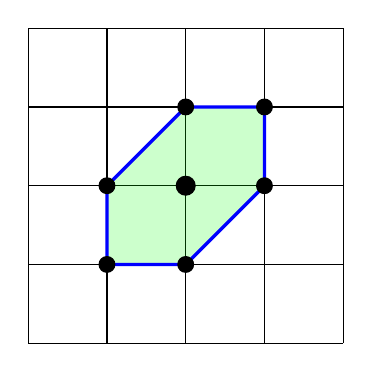
\begin{tikzpicture}
  \draw (0, 0) grid (4, 4);  
\draw [very thick, color=blue, fill=green, fill opacity=0.2]
(1,1) -- (2,1) -- (3,2) -- (3,3) -- (2,3) -- (1,2) -- cycle;
\draw [fill=black]  (1, 1) circle (0.1);
\draw [fill=black]  (2, 1) circle (0.1);
\draw [fill=black]  (3, 2) circle (0.1);
\draw [fill=black]  (3, 3) circle (0.1);s
\draw [fill=black]  (2, 3) circle (0.1);
\draw [fill=black]  (1, 2) circle (0.1);
\draw [fill=black]  (2, 2) circle (0.12);
\end{tikzpicture}
\caption{A hexagon.}
\label{fig:hexagon}
\end{figure}

By starring $E_6$ with a vertex, we get a triangulation of the disk. Denote by $\nabla$, the hexagon in  \cref{fig:hexagon}. By Theorem 8.3 and Corollary 8.9 in \cite{sturmfels}, there is a one-one correspondence between unimodular regular triangulations of $\nabla$ and the square-free initial ideals of the toric ideal of $\P(\nabla)$. 

This means that $E_6 \ast \{ pt \}$ smooths to the del Pezzo surface of degree $6$, and also that $\P(E_6)$ smooths to an anticanonical section of $\dP6$. 

\todo{Talk about the join of two del pezzos}

$X_0$.

\section[Smoothings of X0]{Smoothings of $X_0$}

We will exploit the fact that the cone over $\dP6$ have two smoothings two produce two smoothings of $X_0$.
%    \chapter{Mirror symmetry heuristics}
\label{sec:mirrorsym}

    \appendix           % "Chapter" is renamed "Appendix"
    \appendixpage       % Short for \part*{Appendices}

    \chapter{Computer code}
\label{sec:computercode}

Extensive use of computer software such as \MM and SAGE has been invaluable during my work. In this Appendix I collect some computer code for reproducing some of my calculations.

\section{Computing the singular locus}

In some cases, equations simplify significantly in affine charts. Therefore, using the naive command \texttt{singularLocus} in \MM often takes unnecessarily long time (and sometimes the computations never finish), as it computes the minors of a very large Jacobian matrix. Restricting to each affine chart, we can use the command \texttt{minimalPresentation} to eliminate variables to produce a new ring isomorphic to the first one, but with fewer equations.

The following code produces a list of the components of the singular locus of the projective scheme with ideal $I$.

\begin{lstlisting}[language=Macaulay2]
fastSingularities = I -> (
    R := ring I;
    n := numgens R;breaklines=true,
    gensR := gens R;
    singlist := {};
    for i from 0 to (n-1) do {
        affineChart := I + ideal(gensR_i - 1);
        sing        := radical ideal mingens ideal singularLocus minimalPresentation affineChart;
        inv         := affineChart.cache.minimalPresentationMap;
        singlist = singlist | {(homogenize(preimage(inv,sing),gensR_i))};
        };
    saturate intersect(singlist)
    )
\end{lstlisting}

The method works by computing the singular locus in each affine chart, taking the radical, and then pulling back to the homogeneous coordinate ring. Finally, we get a list of singular loci in each affine chart. We return the (saturation of) the intersection of the singular loci of the affine charts.

It is especially fast when computing the singular locus of toric varieties with low-dimensional singularities.

The following code finds the singular locus of the projectice cone $\overline(C(\P^2 \times \P^2)) \subset \P^9$.

\begin{lstlisting}[language=Macaulay2]
R = QQ[x_0..x_8,x_9]
M = genericMatrix(R,3,3)
I = minors(2,M)
time fastSingularities I
time radical ideal singularLocus I
\end{lstlisting}

Our function performs significantly faster. On a modern Mac, the times are 1.14 seconds versus 4.31 seconds, respectively.

Here is a more involved example. Let $Y'$ be four-dimensional toric variety from Chapter 4. It is defined by the $2 \times 2$-minors two matrices. In \MM we can define it as follows:
\begin{lstlisting}[language=Macaulay2]
S = QQ[x_1..x_6,z_1..z_6,y]
M1 = matrix{{y,x_1,x_2},{x_4,y,x_3},{x_5,x_6,y}}
M2 = matrix{{y,z_1,z_2},{z_4,y,z_3},{z_5,z_6,y}}
J = minors(2,M1) + minors(2,M2)
\end{lstlisting}

Here the performance difference is even more impressive. Our function computes the singular locus in 7.29 seconds, but the built-in function \texttt{singularLocus} used more than 22 minutes (at which point I interrupted the computation).

\section{Torus action}

The following lines checks if a projective scheme with ideal sheaf \texttt{IX} admits an action of a subtorus of $G=(\C^\ast)^n \subset \P^n$. To check this, we check if the equations are still valid after a torus action. Since $G$ is abelian, it act on functions by $\lambda \cdot f(x_1,\ldots,x_n)=f(\lambda_1 x_1, \ldots, \lambda_n x_n)$. 


\begin{lemma}
Suppose $\{ f_1,\ldots, f_r \}$ is a homogeneous generating set for $I_X=\text{\texttt{IX}}$. Then subgroup of $G$ acting on $X \subset \P^n$ is generated by those $\lambda \in G$ such that $\lambda \cdot f_i  = c f_i$ for some $c \in \C^\ast$.
\end{lemma}
\begin{proof}
Let $H$ be the subgroup of $G$ fixing the ideal $I_X$. Let $H'$ be the subgroup of $g \in G$ acting on the $f_i$ by scalar multiplication: $g \cdot f_i =c f_i$. Clearly $H' \subseteq H$.  Now suppose $g \in H$. Then
$$
g \cdot f_1 = \sum_j a_j f_j
$$
for some constants $a_j$. Now $g \cdot f_1 = f_1(\lambda_1 x _1 ,\ldots, \lambda_n x_n)$. Suppose the leading term of $f_1$ is $x_1^{a_1}\cdots x_n^{a_n}$. Then comparing leading terms in the left hand side and the right hand side, we see that $a_1 = \lambda_1^{a_1}\cdots \lambda_n^{a_n} := \lambda^m$. Hence the right hand side is $\lambda^m f_1 + \text{other terms}$. But now there are the same number of terms on each side of the equation, so there are no other terms. Hence $H=H'$. 
\end{proof}

It follows that to find the subgroup of $G$ acting on $X$, we have to find the $\lambda \in G$ such that the $f_i$ are simultaneous eigenvectors for them.

\begin{example}
Let  $X$ be defined by $f = x_0x_1x_2x_3x_4+\sum_{i=0}^5 x_i^5$ in $\P^4$. Then for $\C^4$ to act on it, we must have $\lambda_0\lambda_1\lambda_2\lambda_3\lambda_4=\lambda_0^5=\ldots=\lambda_4^5$. By stting $\lambda_0=1$, we see that all the $\lambda_i$ are the fifth roots of unity. Hence the subgroup acting on $H$ is the subgroup of $\Z/5^5/Z_5$ given by $\{ (a_0,\ldots,a_5) \mid \sum a_i = 0 \}$.
\end{example}

The following code find the subtoruses of $G$ acting on $X$ in this way, by equating terms in the polynomials defining $X$.

\begin{lstlisting}[language=Macaulay2]
loadPackage "Binomials"
torus = ideal apply(flatten apply(apply(apply(flatten entries gens IX, monomials), v ->  flatten entries v), j -> subsets(j,2)),    s -> s_0-s_1)
toruskomps = BPD torus
toruskomps = select(toruskomps, I -> dim I == 1)
\end{lstlisting}
\begin{proof}[Explanation]
The ideal \texttt{torus} is the ideal generated by the differences of terms in the polynomials defining $X$. The \MM package \texttt{Binomials} can decompose binomials over cyclic extensions of $\Q$ with the command \texttt{BPD}. Finally, we select the components corresponding to finite subgroups of the torus.

Then we check manually if these actually correspond to non-trivial actions.
\end{proof}


\section{Computing the Gaifullin triangulation}
\label{sec:compute_gaifullin}

Below is a short SAGE script computing the $15$ vertex triangulation of $\C \P^2$ as described in \cite{cp2_15_chess}. The last line returns a \texttt{SimplicialComplex} object in SAGE.

\begin{lstlisting}[language=Python]
#Defines the Klein 4 group.
V4 = PermutationGroup([Permutation("(1,2)(3,4)"),Permutation("(1,3)(2,4)")])

def isValidFace(F):
    '''
    Assumes the first vertex is a permutation.
    Then checks if F satisfies the condition in the
    definition of T.
    '''
    g = F[0]
    for v in (1,2,3,4):
        if (F[g(v)][1] == F[v][1]):
            return False
    return True


# Makes a list of all possible maximal faces of the correct form
candidates = [(g,(1,a1),(2,a2),(3,a3),(4,a4)) for g in V4.list()[1:] for a1 in (1,2,3) for a2 in (1,2,3) for a3 in (1,2,3) for a4 in (1,2,3)]

# Filters out the faces not fullfilling the condition
maximalFacets = filter(lambda F: isValidFace(F), candidates)

# Renames the vertices
S = SimplicialComplex(maximalFacets)
vertexSet = S.vertices()
D = dict([(F,i) for i,F in enumerate(vertexSet)])
renamedMaximalFacets = [[D[v] for v in F] for F in maximalFacets]
SS = SimplicialComplex(renamedMaximalFacets)
\end{lstlisting}

To get the Stanley--Reisner ideal, one can write:
\begin{verbatim}
list(SS.stanley_reisner_ring().defining_ideal().gens())
\end{verbatim}
The returned value is a list of the monomials generating the Stanley--Reisner ideal of $\mathcal T$. This can then be copied into \MM for further computation.



    \backmatter         % Folios in Arabic numerals, unnumbered chapters.

    \printbibliography

\end{document}